\documentclass{beamer}
\usetheme{Singapore}

%\usepackage{pstricks,pst-node,pst-tree}
\usepackage{amssymb,latexsym}
\usepackage{graphicx}
\usepackage{fancyvrb}
\usepackage{hyperref}

\newcommand{\bi}{\begin{itemize}}
\newcommand{\li}{\item}
\newcommand{\ei}{\end{itemize}}
\newcommand{\Show}[1]{\psshadowbox{#1}}


\newcommand{\grf}[2]{\centerline{\includegraphics[width=#1\textwidth]{#2}}}
\newcommand{\tw}{\textwidth}
\newcommand{\bc}{\begin{columns}}
\newcommand{\ec}{\end{columns}}
\newcommand{\cc}[1]{\column{#1\textwidth}}

\newcommand{\bfr}[1]{\begin{frame}[fragile]\frametitle{{ #1 }}}
\newcommand{\efr}{\end{frame}}

\newcommand{\cola}[1]{\begin{columns}\begin{column}{#1\textwidth}}
\newcommand{\colb}[1]{\end{column}\begin{column}{#1\textwidth}}
\newcommand{\colc}{\end{column}\end{columns}}

\title{Notes on Effective Learning}
\author{Based on\\
\href{http://makeitstick.net/}{\bf make it stick}\\
\em The Science of Successful Learning
\\\small Brown, Roediger \& McDaniel, 2014}

\RecustomVerbatimEnvironment{Verbatim}{Verbatim}{frame=single}

\begin{document}
\begin{frame}
\maketitle

\end{frame}

\bfr{}
\begin{quotation}
When you struggle with a problem, that's when you understand it.

Anyone who struggled hard with a problem, never forgets it.

\hfill ---Elon Musk

\hfill CEO, Tesla Motors, SpaceX
\end{quotation}
\end{frame}

\bfr{Learning: you're doing it wrong}
\bi
\li Learning is best when it's {\em effortful}.
\li We are {\em poor judges} of when we are learning well.
\li {\em Rereading text} gives little benefit
but leads to false sense of mastery.
\li {\em Massed practiced}, repeating something over and over
until learned, rarely works.
\ei
\end{frame}

\bfr{Which penny is real?}
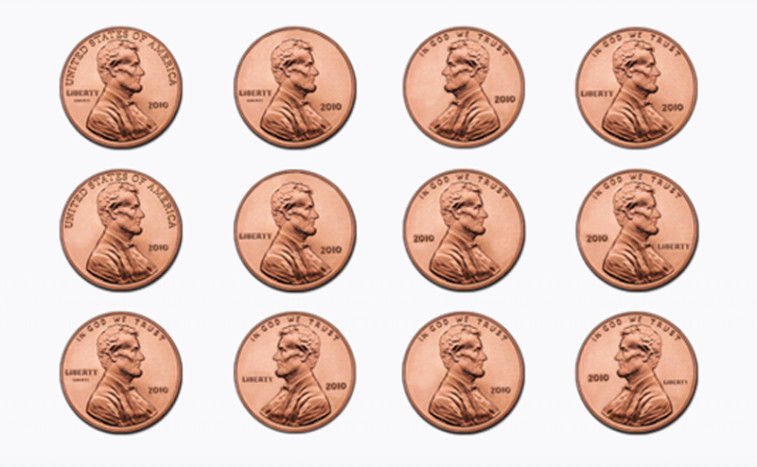
\includegraphics[width=\textwidth]{pennymemorytest.jpg}
\end{frame}

\bfr{Learning: doing it right}
\bi
\li {\em Retrieval practice} is far more effective.
\li Flash cards are the simplest example.
\li Trying to solve a problem yourself
leads to better learning,

\li ... even if you try before you know how
\li ... even if errors are made

\ei
\end{frame}

%\bfr{Learning styles:  NOT}
%\bi
%\li The popular notion that you learn better when you receive
%instruction in a form consistent with your {\em learning style}, for
%example auditory or visual, is {\bf not supported by empirical
%  evidence.} 
%\li People do have multiple learning strategies, and all people learn
%best when they ``go wide.''
%\li Limiting instruction to your preferred style reduces learning.
%\ei
%\end{frame}

%\bfr{Learning rules {\em vs.} learning facts}
%\bi
%\li When you learn underlying principles or {\bf rules} you are more
%adept at picking the right solutions in unfamiliar situations.
%\li This skill is better acquired through {\bf interleaved and varied
%  practice} than massed practice.
%\ei
%\end{frame}

\bfr{We are all susceptible to {\bf illusions} of learning}
\bi
\li Rereading or highlighting 
the text gives the illusion of fluency.
\li {\bf Testing} helps calibrate our judgements.
\li ``Shooting an azimuth.''
\ei
\end{frame}

\bfr{}
\begin{center}
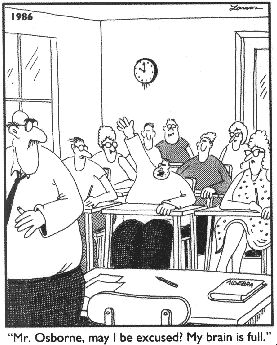
\includegraphics[height=0.9\textheight]{brainisfull.jpg}
\end{center}
\end{frame}

\bfr{There is no known limit to the capacity for learning}
\bi
\li In 2010 Simon Reinhard memorized 300 random words in 15 minutes.
\li In 2008 Ben Pridmore memorized 884 shuffled playing cards in 30 minutes. 
\li In 2010 Boris-Nikolai Konrad memorized 201 names and faces in 15 minutes.
\li {\bf Elaboration} is the practice of putting things in your own words
and connecting it to what you already know.
\ei
\end{frame}

\bfr{Learning changes your brain}
\bi
\li Every time you learn something you {\bf change your brain}.
\li The hippocampus, important in
long-term memory, actually creates new neurons throughout your life.
\li But only if it has to.
\li When learning is hard, you're doing important work.
\ei
\end{frame}

\bfr{The Testing Effect}
\bi
\li Tests: assessment {\em vs.} learning tool
\li Aristotle:  {\em exercise in repeatedly recalling a thing
strengthens the memory}
\ei
\end{frame}

\bfr{An experiment}
\bi
\li Subjects were given passages to read.
\li Some passages were immediately tested on.
\li Other passages were reread.
\li {\bf Tested passages were remembered better.}
\ei
\end{frame}

\bfr{Another experiment}
\bi
\li Some subjects asked to memorize pairs like {\em foot-shoe}
\li Others asked to memorize pairs like {\em foot-s\_\_e}
\li {\bf Second group did substantially better.}
\ei
\end{frame}
\bfr{}
\centerline{\huge\fbox{\sc Quizzing is a learning tool!}}
\end{frame}

\bfr{}
\begin{center}
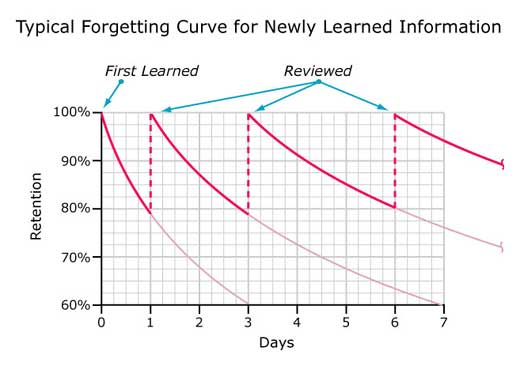
\includegraphics[width=\textwidth]{ForgettingCurve.jpg}
\end{center}
\end{frame}


\bfr{How to practice retrieving from memory}
\bi
\li Quiz, quiz, quiz!
\li Use flash cards: \url{www.ankisrs.net}
\li Use Cornell note taking system \\\url{http://lsc.cornell.edu/LSC_Resources/cornellsystem.pdf}
\li Look up from the book and summarize
\li Invent quiz questions as you read
\ei
\bi
\li Don't listen to your intuition!  Shoot an azimuth!
\li Space out retrieval practice, no cramming.
\ei
\end{frame}

\bfr{Relate it to your own experience}

\begin{description}
\item[Generation:]
  Try to answer a problem before being shown the solution
\item[Elaboration:]
  Explain it in your own words and relate it to your own experience
\item[Reflection:] Write out essays on your learning
\end{description}
\end{frame}


\bfr{}
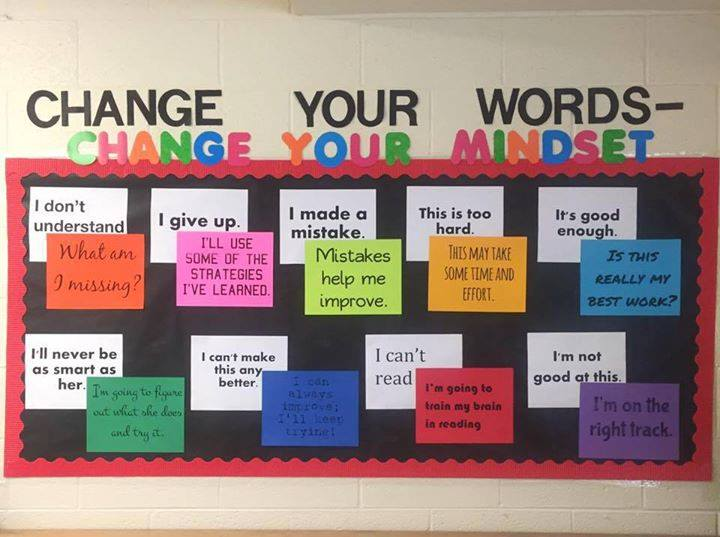
\includegraphics[width=\textwidth]{changeyourvocabulary.jpg}
\end{frame}

\bfr{}

\LARGE 
\begin{quotation}
We are what we repeatedly do. Excellence, then, is not an act, but a habit.

\hfill ---Aristotle
\end{quotation}

\end{frame}

\end{document}
